\documentclass{beamer}
\usetheme{default}
\setbeamertemplate{navigation symbols}{}
%	
\usepackage{subfig}
\usepackage{epstopdf}
\usepackage{amsmath, amsthm, amssymb}
\usepackage{float}
\usepackage{rotating}
\usepackage{graphicx}
\usepackage{longtable}
\usepackage{xcolor}
\usepackage{bm}
\usepackage{tikz}
\usetikzlibrary{shapes}
\newcommand{\EE}{\mathbb E}
\newcommand{\var}{\mathrm{var}}
\newcommand{\cov}{\mathrm{cov}}
\newtheorem{acknowledgement}[theorem]{Acknowledgement}
\newtheorem{algorithm}[theorem]{Algorithm}
\newtheorem{assumption}{Assumption}
\newtheorem{axiom}{Axiom}
\newtheorem{case}[theorem]{Case}
\newtheorem{claim}[theorem]{Claim}
\newtheorem{conclusion}[theorem]{Conclusion}
\newtheorem{condition}[theorem]{Condition}
\newtheorem{conjecture}{Conjecture}
\newtheorem{criterion}[theorem]{Criterion}
\newtheorem{proposition}{Proposition}
\newtheorem{summary}[theorem]{Summary}
\newtheorem{exercise}{Exercise}
\newtheorem{notation}{Notation}
\newtheorem{remark}{Remark}
%\graphicspath{{graphs//}}

\title {BEGS: Quantitative Results}

\date{September 2013}
% \today will show current date.
% Alternatively, you can specify a date.
%
\begin{document}
%
\begin{frame}
\titlepage

\end{frame}


\begin{frame}
\frametitle{Numerical exercise}
 
Solve a $N=5$ agent economy with realistic level and movements in wage dispersion across booms and recessions

\begin{itemize}
 \item Long run dynamics: Study settings that differ in covariance of interest rates and output
 \item Transient dynamics: Study outcomes in recessions that are accompanied by higher inequality
\end{itemize}

Aggregate shocks affect,
\begin{enumerate}
\item Wages: \[\log \theta_i=\epsilon [1+(.9-i)m]\]
 \item Payoffs: \[P=1+\chi \epsilon \]
\end{enumerate}

\end{frame}

\begin{frame}
\frametitle{Calibration}

\begin{table}[htp]
\small
\begin{tabular}{|l|c|p{4cm}|}
\hline
Parameter & Value & Description   \\ \hline
$\{\bar{\theta}_i\} $ & \{1 ,  1.4,  2.1,  3.24,  4.9\} & Wages dispersion for \{10,25,50,75,90\} percentiles   \\
$\gamma$ & 2 & Average Frisch elasticity of labor supply of 0.5 \\
$\beta$ & 0.98  &Average (annual) risk free interest rate of 2\%   \\
$m$ &$\frac{1.5}{.8}$& Changes in dispersion \\
$\chi$ & -0.06 &covariance between holding period returns and labor productivity\% \\
$\sigma_e$ & 0.03 & vol of labor productivity\\
$g$ & .13 \%&Average pre-transfer expenditure- output ratio of 12 \% \\\hline
\end{tabular}
\caption{Benchmark calibration}
\label{tab:Parameters}
\end{table}
\small
The Pareo weights and initial distribution of wealth is chosen to match an average tax rate of $20\%$ and debt to gdp ratio of $100\%$ and transfers to gdp ratio of 10\% and deciles of US wealth distribution
\end{frame}
\begin{frame}
 \frametitle{Calibration: Interest rates}
 Let $q^{(n)}_t$ be the log price of a nominal bond of maturity $n$. We can define the real holding period returns $r^{(n)}_{t,t+1}$ as follows
 
 \[r^{(n)}_{t,t+1}= q^{(n-1)}_{t+1}-q_t^{(n)}-\pi_{t+1}\]
 With the transfromation $y^{(n)}_t: -\frac{1}{n} q^{(n)}_t$ we can express $r^{(n)}_{t,t+1}$ as follows:
 \small
 \[r^{(n)}_{t,t+1}=\underbrace{y^{(n)}_t}_{\text{Ex-ante part}} - (n-1)\left[\underbrace{\left(y^{(n)}_{t+1}-y^{(n)}_{t}\right)}_{\text{Interest rate risk given $n$}}+\underbrace{\left(y^{(n-1)}_{t+1}-y^{(n)}_{t+1}\right)}_{\text{Term structure risk}}\right]-\underbrace{\pi_{t+1}}_{\text{Inflation risk}}\]
\end{frame}


\begin{frame}
 \frametitle{Calibration: Interest rates}
 \small
 \begin{itemize}
  \item In the model the holding period returns are given by $\log\left[\frac{P_{t+1}}{Q_{t}}\right]$ and $Q_t=\frac{\beta \mathbb{E}_tu_{c,t+1}P_{t+1}}{u_{c,t}}$. 
\item $P_{t+1}$ allows us to captures ex-post fluctuations in returns to the government's debt  portfolio coming from maturity and inflation. 
\item Since $\epsilon_{t}$ is i.i.d over time in our calibration  $\chi=\frac{\sigma_{r}}{\sigma_{\epsilon}} Corr(r,\epsilon)$
 \end{itemize}

 Using data on labor productivity $\epsilon_{t}$ and $\{q^{n}_t\}_{n}$ we can compute the correlation table as follows:
 
\begin{table}[htp]
\small
\begin{tabular}{|l|l| l|l|l|}
\hline
Maturity (n) &2yr & 3yr & 4yr & 5yr\\
\hline
$Corr(\epsilon_{t+1},r^{(n)}_{t,t+1})$ & -0.11 &-0.093 &-0.083 &-0.072\\
$Corr(\epsilon_{t+1},r^{(n)}_{t,t+1}-ny^{(n)}_{t})$& 0.00 & -0.0463 &-0.080& -0.091\\
$Corr(\epsilon_{t+1},y^{(n)}_{t}-\pi_{t+1})$ &-0.097  &-0.086  &-0.080  &-0.073 \\ 
\hline
\end{tabular}
\caption{}
\label{tab:corr}
\end{table}
Further $Corr(\epsilon_{t+1},\pi_{t+1})=0.068$ and for 3 month real tbill returns $Corr(\epsilon_{t+1},y^{1 qtr}_{t}-\pi_{t+1})=-0.11$
 
\end{frame}




\begin{frame}
\frametitle{Long run}
 {
  \begin{figure}
    \centering
    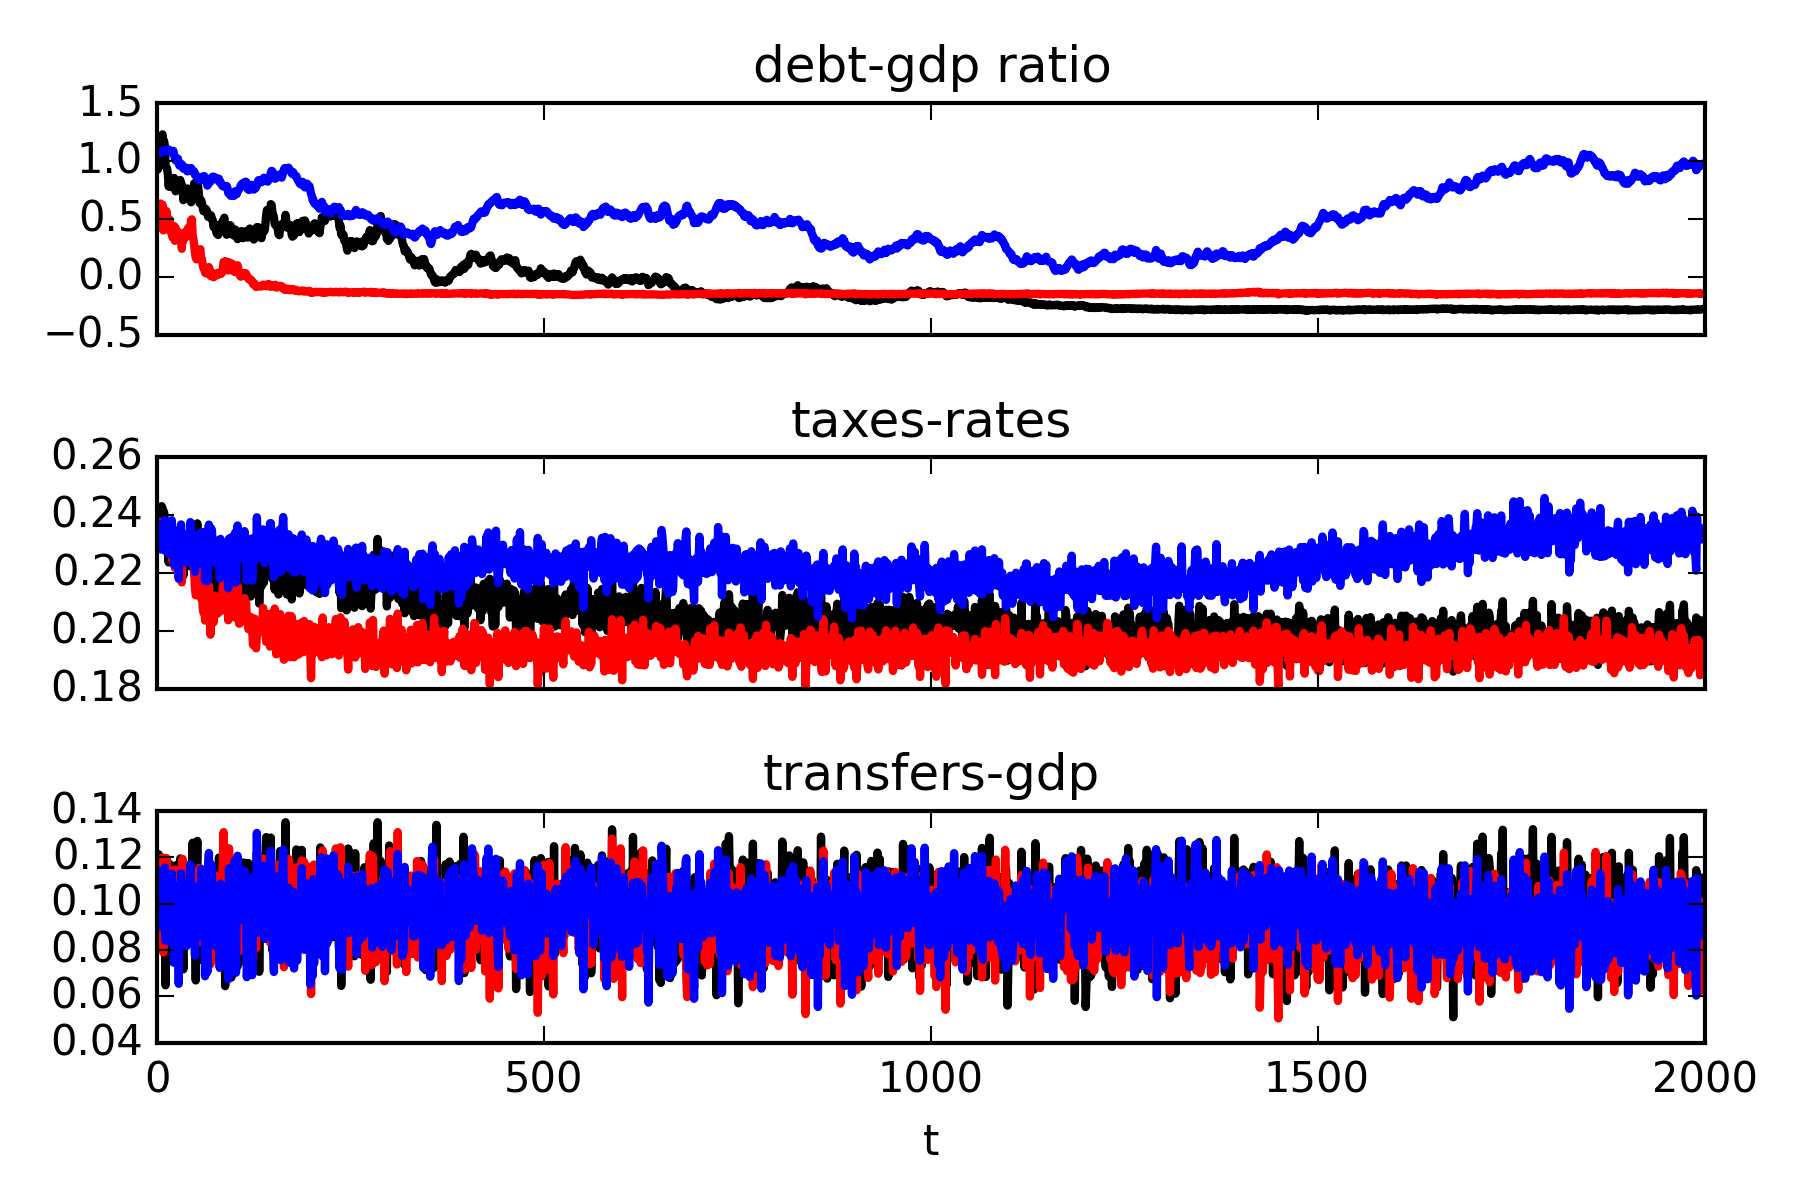
\includegraphics[width = 0.9\textwidth]{cesplots/long_simulation_debt.png}
    \caption{The red, black and blue lines plot simulations for a common sequence of shocks for values of $\chi=-1.5,0,1.5$ respectively}
  \end{figure}

}

\end{frame}


\begin{frame}
\frametitle{Long run: Speed of convergence}
 {
  \begin{figure}
    \centering
    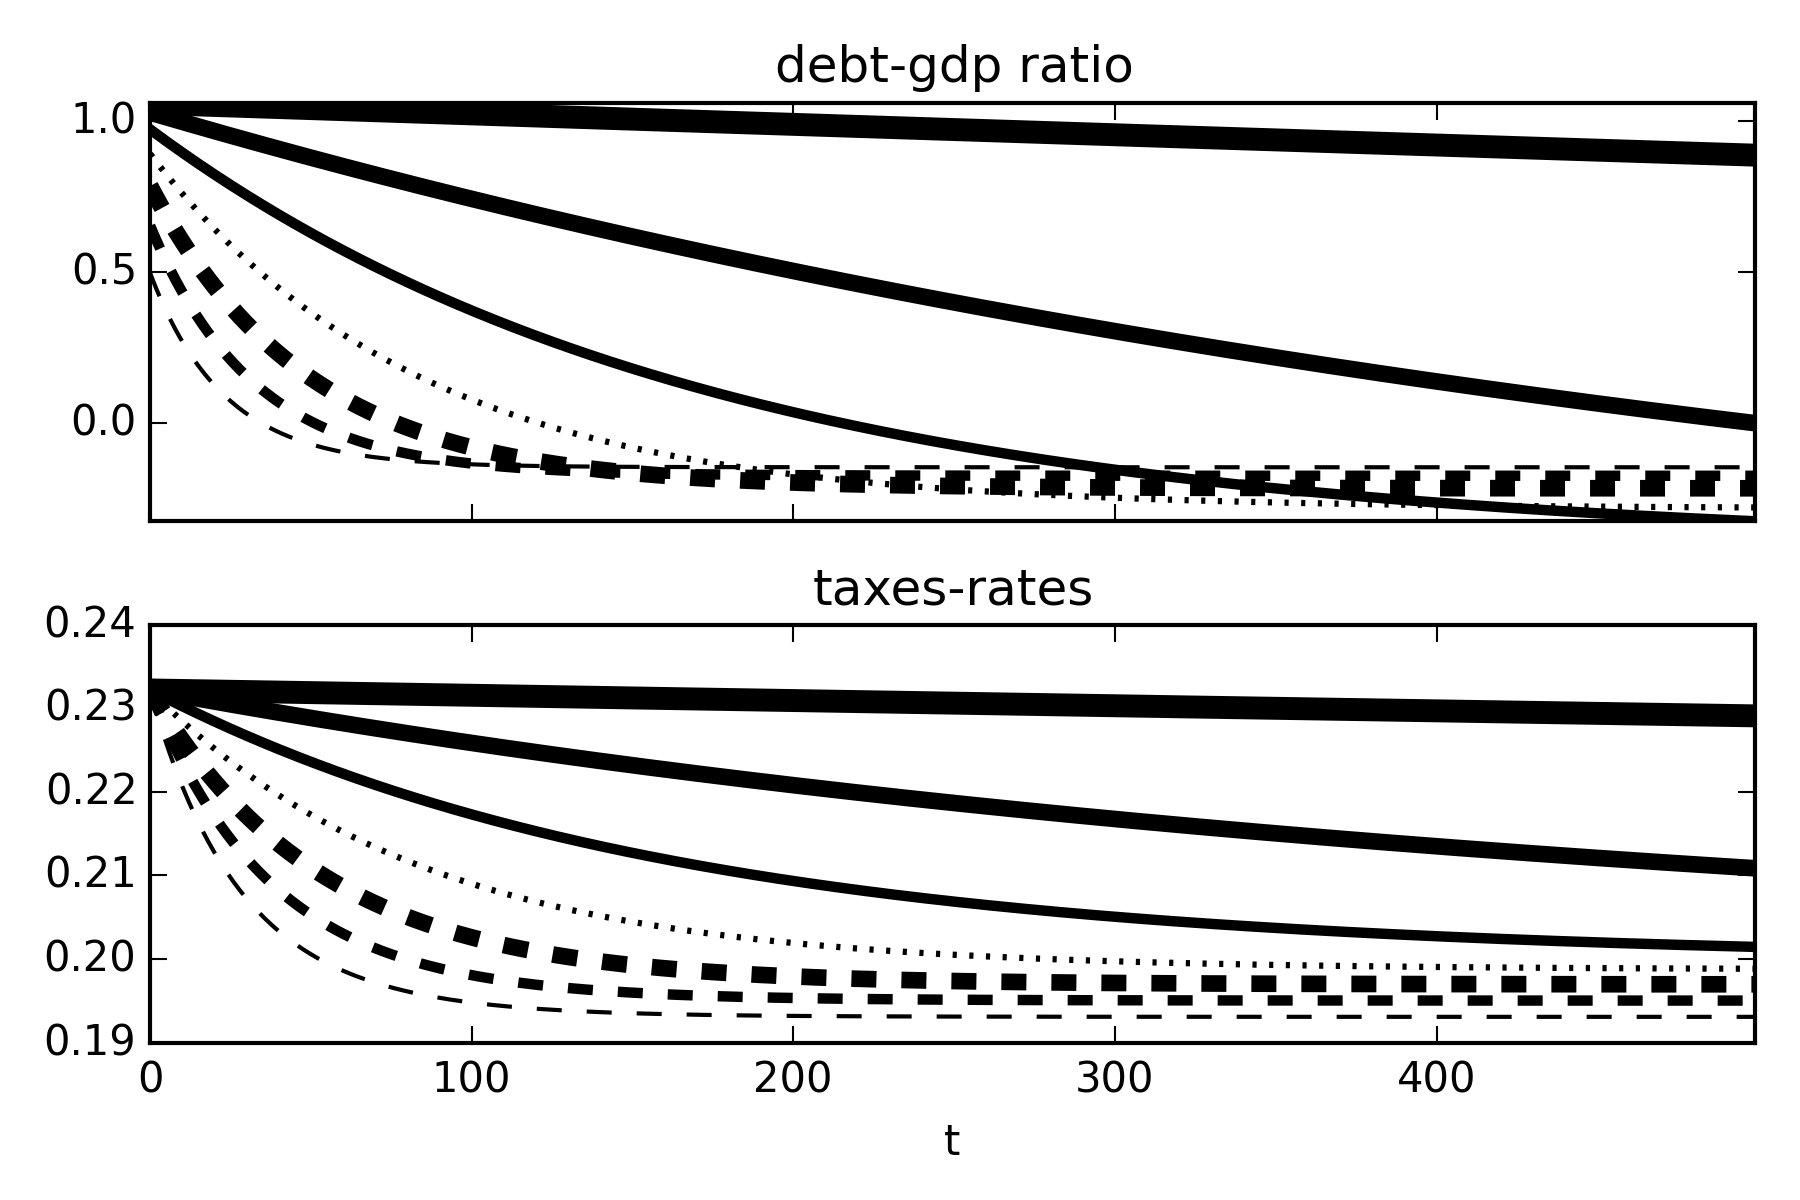
\includegraphics[width = 1.0\textwidth]{cesplots/speed_of_convergence.png}
    \caption{The plot shows conditional mean paths for different values of $\chi$. The red (blue) lines have $\chi<0$ ($\chi>0$). The thicker lines represent larger values.}
  \end{figure}

}

\end{frame}

\begin{frame}
 \frametitle{Spreading of taxes}
{
  \begin{figure}
    \centering
    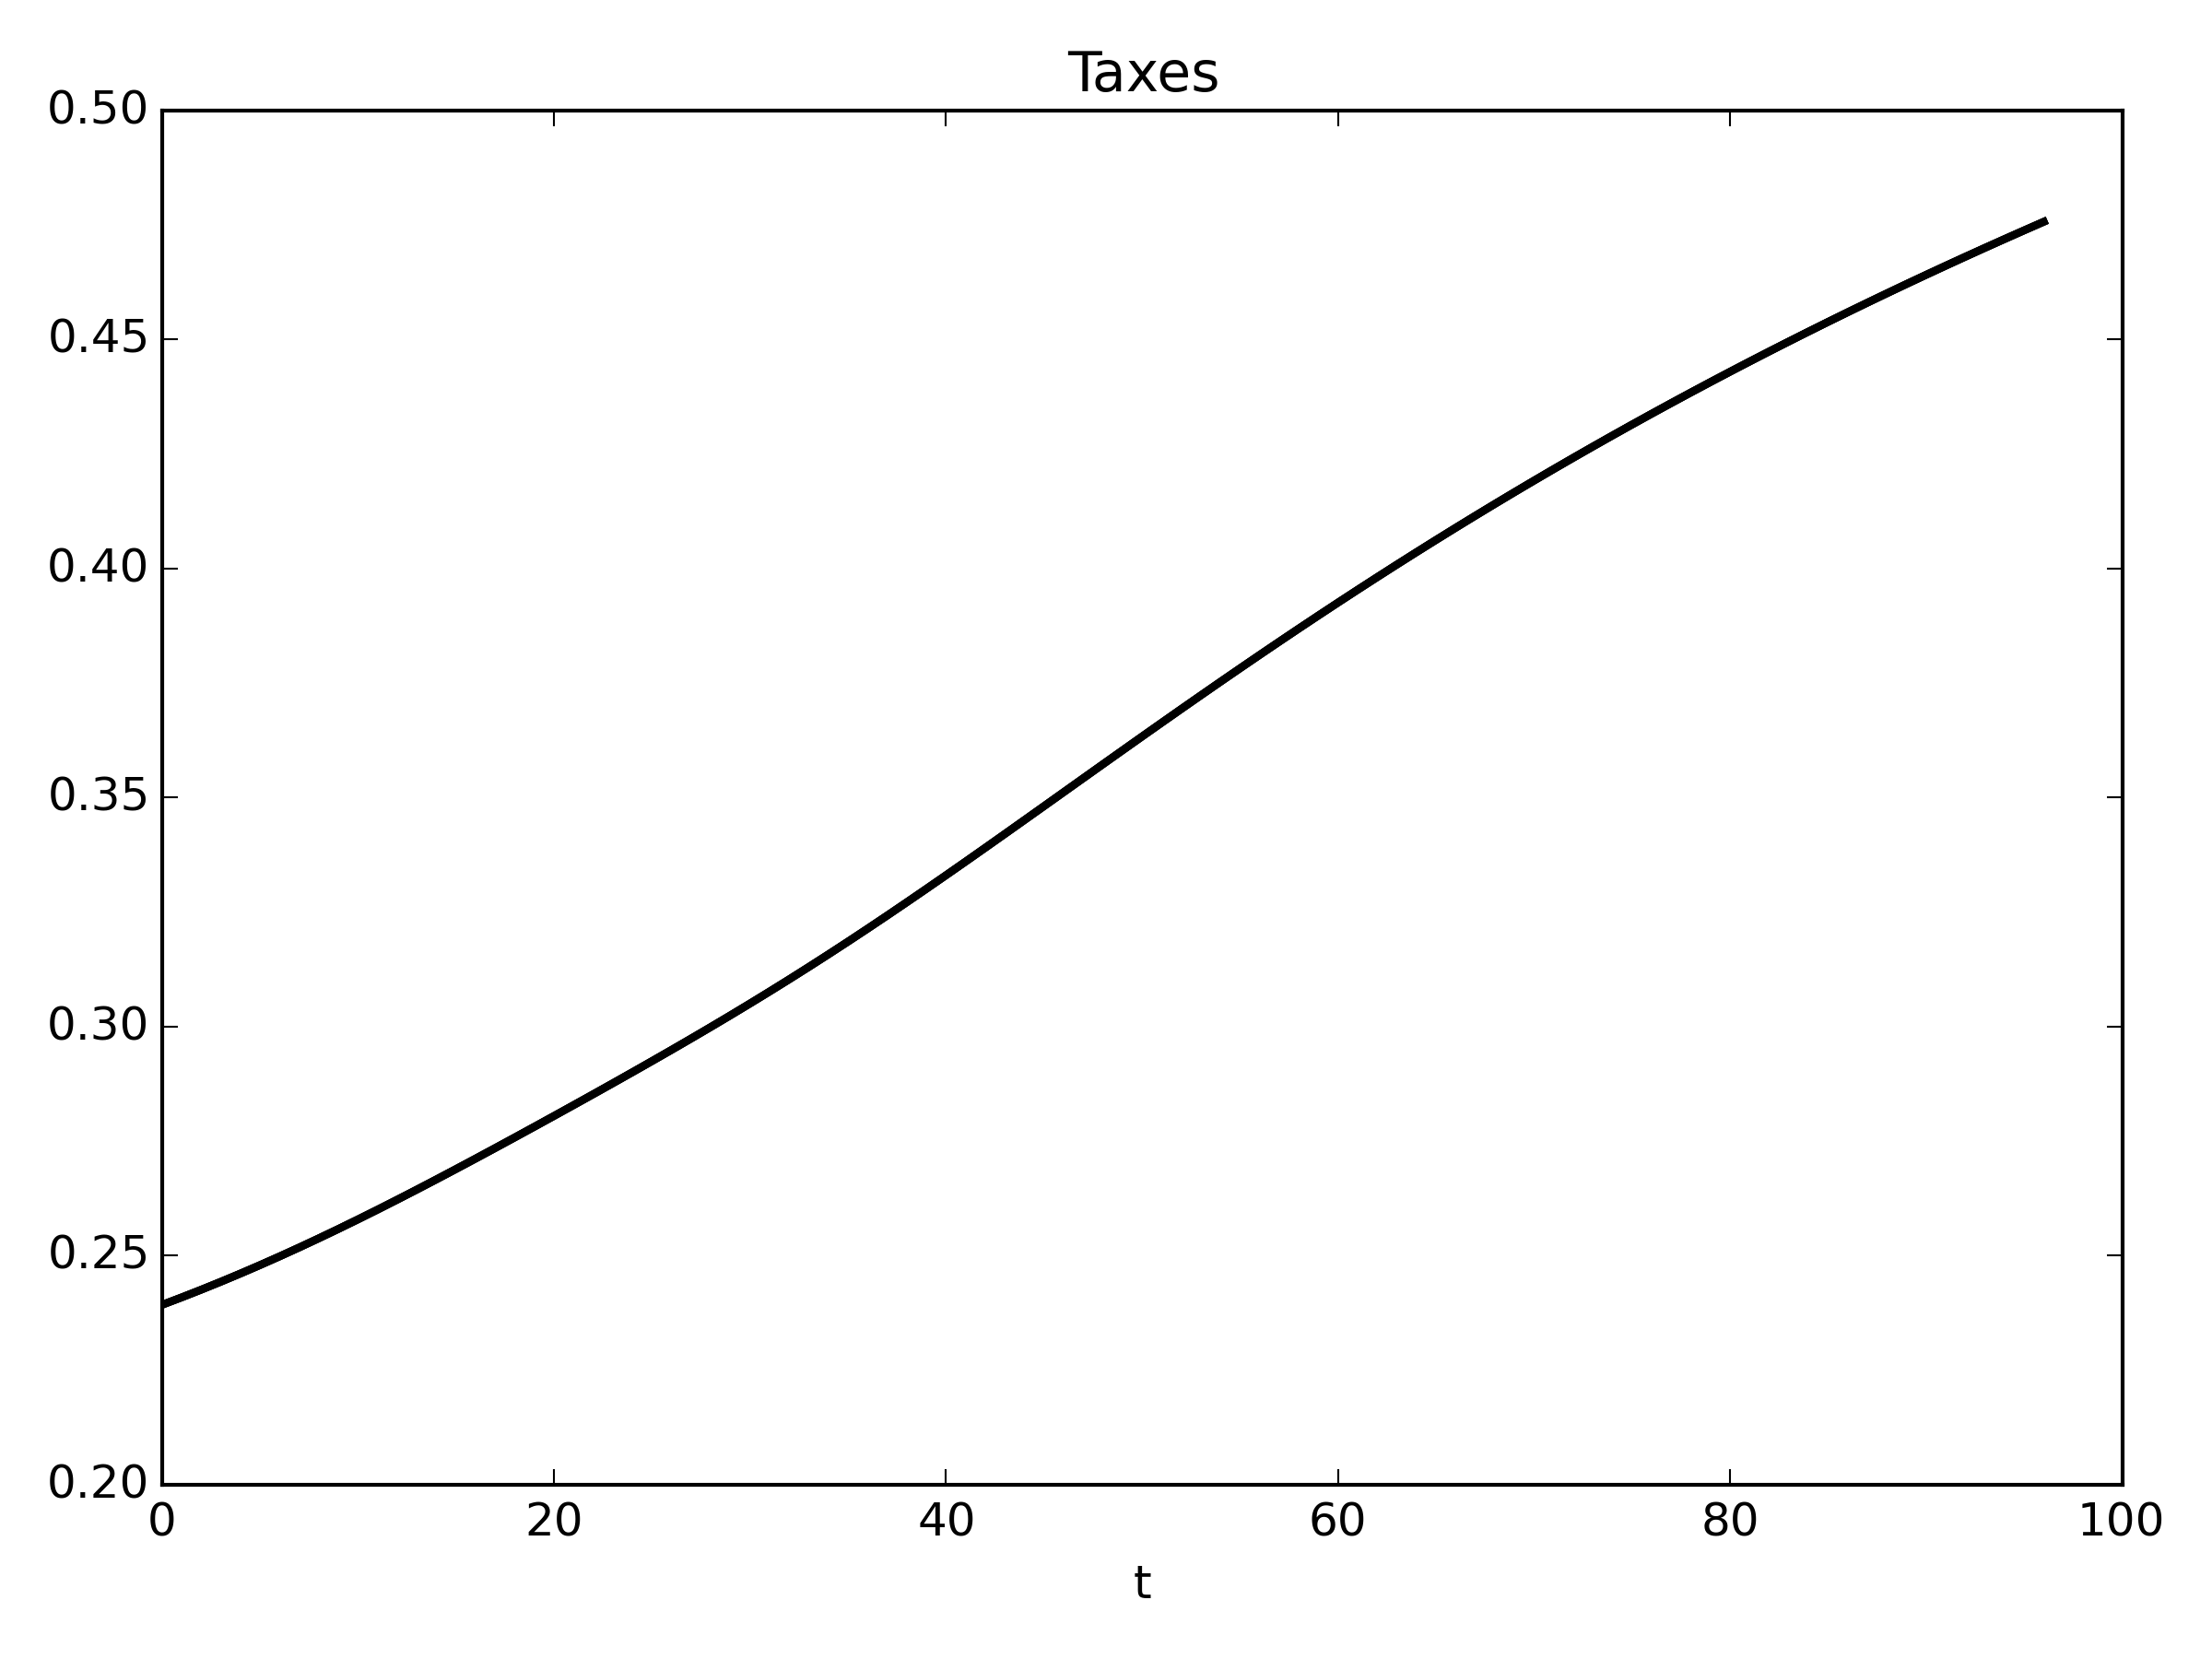
\includegraphics[width = 0.9\textwidth]{cesplots/taxes_only_bad_shocks.png}
    \caption{Taxes for a sequence of -1 s.d shocks to aggregate productivity}
  \end{figure}

} 
 
\end{frame}


\begin{frame}
\frametitle{Short run}
Lets denote consecutive period of negative (positive) one s.d $\epsilon$ shocks a ``recession'' (boom)

\begin{itemize}
\item Simulate a recession that is followed by no further shocks
 
 \item Decompose responses into TFP component and inequality component:
  
 \vspace{3mm}
\centering  \textbf{Baseline:} $\log \theta_i=\epsilon [1+(.9-i)m]$
 \vspace{3mm}
 \begin{itemize}
  \item Only TFP: \[\log \theta_i=\epsilon\]
  \item Only Ineq: \[\log \theta_i=\epsilon [(.9-i)m]\]
\end{itemize}

\end{itemize}
 
\end{frame}


\begin{frame}
\frametitle{Recessions with higher inequality}
{
  \begin{figure}
    \centering
    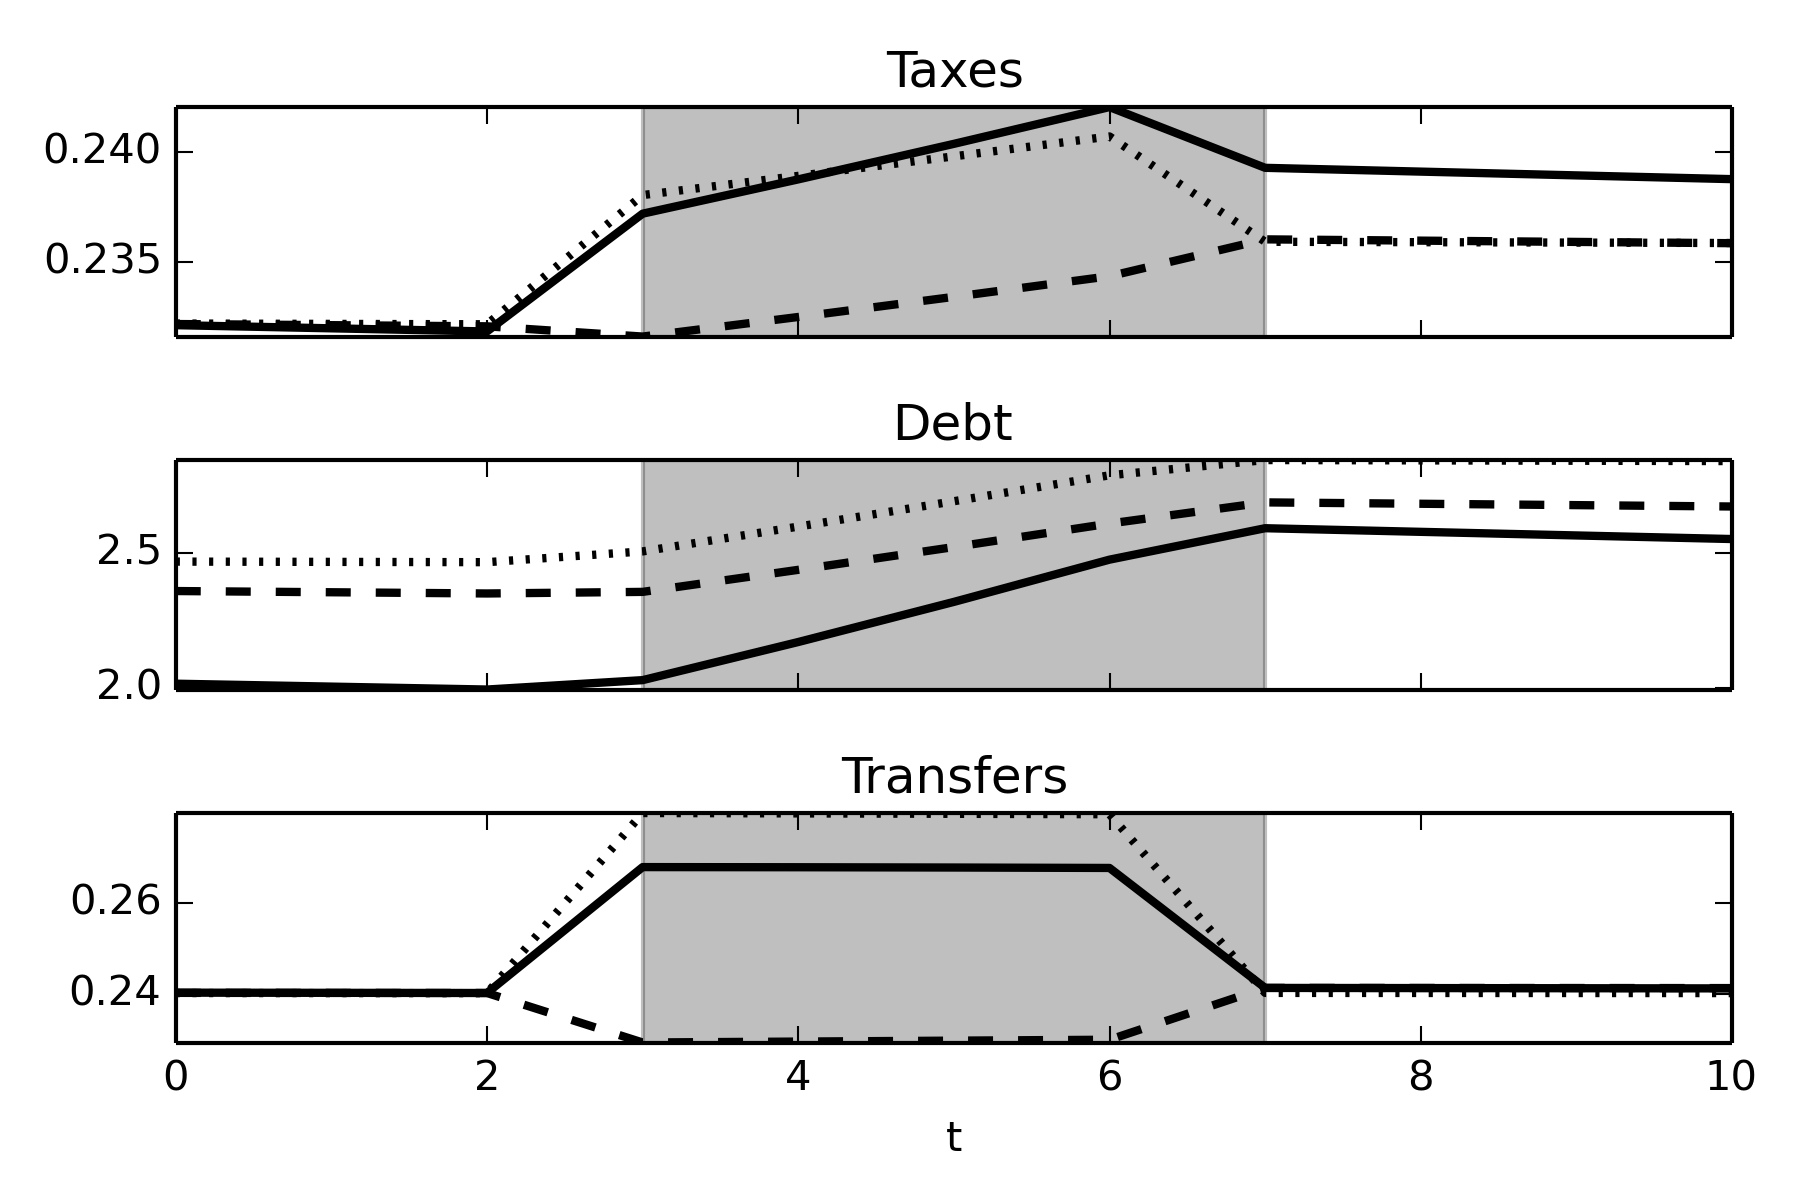
\includegraphics[width = 0.9\textwidth]{cesplots/irf_bm_chi_shocks.png}
    \caption{The bold line is the total response. The dashed (dotted) line reflects the only TFP (inequality) effect. The shaded region is the recession}
  \end{figure}

} 
\end{frame}





\begin{frame}
\frametitle{Tfp and Tfp+Ineq recessions: Sample moments}
\begin{table}[htp]
\small
\begin{tabular}{|l|l|l|}
\hline
Moments &Tfp& Tfp+Ineq\\\hline
vol. of taxes & 0.003&0.006\\
vol. of transfers &0.01 &0.02\\
autocorr. in taxes& 0.93&0.66\\
autocorr. in transfers& 0.17&0.18\\
corr. of taxes with tfp &0.15 &-0.63\\
corr. of transfers with tfp & 0.99&-0.98\\ \hline
\end{tabular}
\caption{These are sample moments averaged acrosss simulations of 100 periods}
\label{tab:corr}
\end{table}

\end{frame}


\begin{frame}
\frametitle{Redistribution in recessions}
\begin{itemize}
 \item TFP : Relative inequality is unchanged and planner redistributes by lowering tax-rates on impact.
 \item Only Ineq : Earnings gap increases by factor $m$. The planner mainly redistributes mainly through higher transfers and taxes.
 \item TFP + Ineq: For both tax rates and transfers are higher. Relative to the Tfp case the volatility of taxes and trasnfers is twice as much.
\end{itemize}
\end{frame}


 \end{document}